\lstinputlisting[language=bash,basicstyle=\small]{python_codes/fieldstone_60/keywords}

This stone implements the 1D discontinuous Galerkin method to solve the simple 
advection equation:
\[
\frac{\partial T}{\partial t} + u \frac{\partial T}{\partial x} = 0
\]




%---------------------------------------------
\subsection*{The code}

The mesh counts {\tt nelx} linear elements and therefore {\tt nnx} nodes.

The timestep is determined by means of the CFL condition:
\begin{lstlisting}
dt=C*hx/u
\end{lstlisting}
The mesh is very simply built:
\begin{lstlisting}
x=np.linspace(0,Lx,nnx)
\end{lstlisting}
We need to declare four arrays: the nodal temperature both on the left and 
on the right of each node, and their memory of the previous time step. 
\begin{lstlisting}
T_minus=np.zeros(nnx,dtype=np.float64)      
T_minus_old=np.zeros(nnx,dtype=np.float64)  
T_plus=np.zeros(nnx,dtype=np.float64)       
T_plus_old=np.zeros(nnx,dtype=np.float64)   
\end{lstlisting}
Initial temperatures are then prescribed on both {\tt T\_plus} 
and $T\_minus$ arrays, and then copied to the 'old' arrays.

We then enter the time stepping loop:
\begin{lstlisting}
for istep in range(0,nstep):
\end{lstlisting}
At each timestep the boundary conditions are reapplied\footnote{It is a bit weird that 
we prescribe a temperature b.c. on a node with an outflow...?}:
\begin{lstlisting}
T_minus[0]=T_left
T_plus[0]=T_left
T_minus[nnx-1]=T_right
T_plus[nnx-1]=T_right
\end{lstlisting}
We then loop over all elements:
\begin{lstlisting}
for iel in range(0,nel):
\end{lstlisting}
and compute the corresponding $k$ and $k+1$ values:
\begin{lstlisting}
k=iel
kp1=iel+1
\end{lstlisting}
The $T^+$ and $T^-$ fields are then updated following Eq.~\eqref{eq:dgadv5}:
\begin{lstlisting}
T_plus[k]   =T_plus_old[k]   +C*(-3*T_plus_old[k]-T_minus_old[k+1]+4*T_minus[k])
T_minus[k+1]=T_minus_old[k+1]+C*( 3*T_plus_old[k]-T_minus_old[k+1]-2*T_minus[k])
\end{lstlisting}







%---------------------------------------------
\subsection*{Results}

%---------------------------------------------
\subsubsection*{Experiment 1}

We consider the following advection problem taken from Li \cite[ex 5.2]{li06}.
It is also carried out in \stone~43.

The domain has dimension $L_x=1$. 
The temperature is prescribed on the left and the right boundary to be zero. 
The initial temperature is given by
\[
T(x,0)=
\left\{
\begin{array}{ll}
\sin (10 \pi x) & \textrm{for } x< 0.1 \\
0               & \textrm{for } x\geq 0.1 
\end{array}
\right.
\]
The velocity is set to $u=0.1$.
We use 200 elements and a time step of $\delta t=10^{-4}$. 
We run the model to time $t=8$ so we need 80,000 time stpes. 

Note that the CFL-number is then very small: 
\[
C = \frac{\delta t \cdot u}{h} = \frac{10^{-4} \cdot  0.1}{1/200} = 0.002
\]

\begin{center}
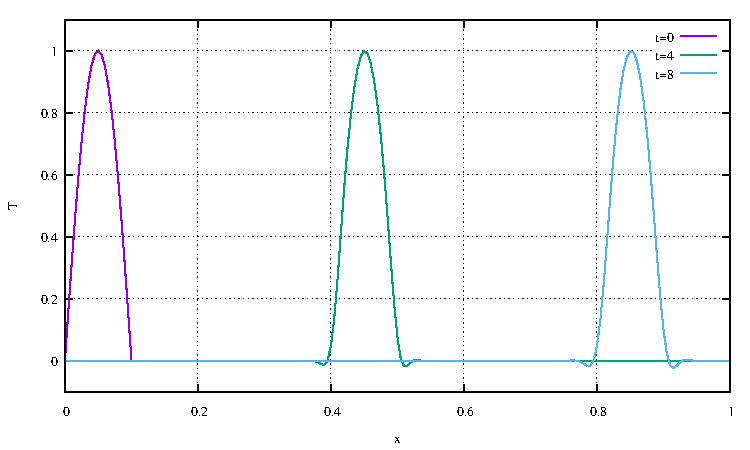
\includegraphics[width=9cm]{python_codes/fieldstone_60/results/exp1/T.pdf}\\
{\captionfont Temperature field at three different times.}
\end{center}

\todo[inline]{redo with standard Galerkin and compare!}

%---------------------------------------------
\subsubsection*{Experiment 2}

This advection benchmark originates in Donea \& Huerta \cite{dohu03}
and it also to be found in Thieulot (2011) \cite{thie11} (and in 
Section~\ref{ss:appAthie11}).

The domain has dimension $L_x=1$. 
The temperature is prescribed on the left at $T=1$
and the right boundary at $T=0$.
The initial temperature is given by
\[
T(x,0)=
\left\{
\begin{array}{ll}
1 & \textrm{for } x< 0.25 \\
0 & \textrm{for } x\geq 0.1 
\end{array}
\right.
\]
Velocity is set to $u=1$, the number of elements to 50 ($h=0.02$), the CFL number to 0.1 (
so $\delta t=0.002$), and the number of time steps to 250, so that we expect the front
to be at $x=3L_x/4$.  

\begin{center}
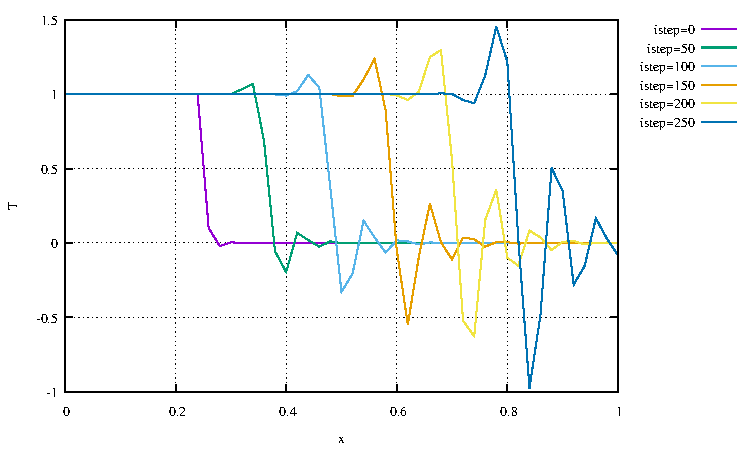
\includegraphics[width=8cm]{python_codes/fieldstone_60/results/exp2/T.pdf}\\
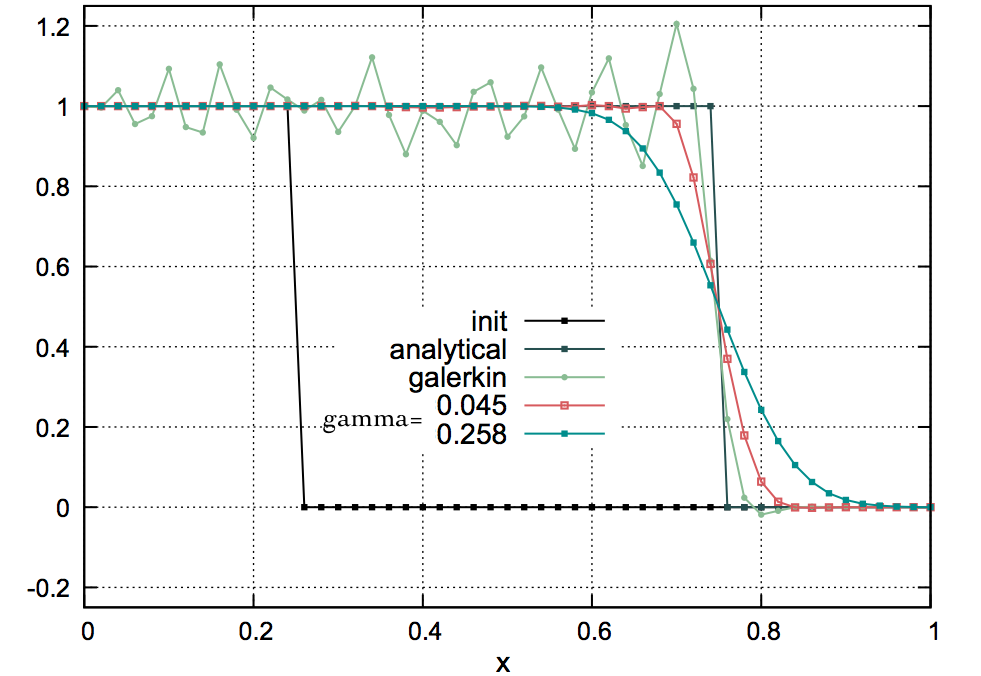
\includegraphics[width=8cm]{images/supg/fantom3}\\
{\captionfont Left: Temperature field at different times; 
Right: Taken and modified from Thieulot (2011) \cite{thie11}}
\end{center}

It is rather surprising that the DG results are so much worse than the SG results (even without 
SUPG stabilisation).









